\section{Performance and Bechmarking}
\label{Chapter:Performance}

\subsection{Characterization}
An important aspect of fabricating a new technique is measuring how well it performs in different usage scenarios. Developing a metrics for judging the artistic quality of a calligraphy specimen produced by the Bezier or rotating Bezier splines is altogether a separate discussion and out of scope of this research. However, there are some aspects that we have tried to measure the effectiveness of the rotating splines.

\subsection{Supported Scripts}
All the scripts that are written with rigid broad-edge tools, such as broad-edge pens and markers, where the tool keeps complete contact with the surface throughout the stoke. However, if script requires changing the extent of tool contact with the surface, the best alternate to achieve a similar appearance of the script would be to use multiple splines with multiple thicknesses that overlap each other in a gradual manner. The rotating bezier splines cannot control the tool inclination and applied pressure, therefore, they are not suitable for scripts written with flexible tools like broad-edge brushes.

\subsubsection{Coverage}
To benchmark the performance and accuracy of rotating bezier splines, some test results are presented here. These values are produced by comparing high resolution binary images of actual scripts, extracted with Adobe Photoshop and rasterized images produced by the twisting bezier splines originally formed by tracing the processed images. The pixel density is set such that a pixel-pixel comparison can be performed between the original image and the rasterized splines. The accuracy is analysed by computing the overflow and underflow of the ink by matching pixels of both images. Table \ref{Table:Accuracy} shows a summary of these benchmarks.

\begin{table}
\begin{center}
\caption{Benchmark of the mathematical accuracy of the twisting bezier spline curves}
\label{Table:Accuracy}
\begin{tabular}{| c | c |}
  \hline
\textbf{Metrics} & \textbf{Results} \\
  \hline
Area over flow & $<$ 2\% \\
  \hline
Coverage & $>$ $94\%$ \\
  \hline
Lateral deviation from the pitch line & N.A. \\
  \hline
Compatibility & All broad edge scripts \\
  \hline
Total splines measured & $>100$ \\
  \hline
Total pixels compared & $9.9$~million \\
  \hline
Tested scripts & Nastaleeq, Thuluth \\
\hline
\end{tabular}
\end{center}
\end{table}
%
%This metrics is comprehensive but still not complete. Some additional metrices are still needed to give a verdict about how good the proposed solution is and it is now up to the community to evolve these curves according to the needs. Table \ref{Table:AdvancedMetrices} presents a couple of those metrices that may also be desired by the researchers.
%
%\begin{table}
%\begin{center}
%\caption{Advanced metrices to gauge the effectiveness of twisting bezier splines.}
%\label{Table:AdvancedMetrices}
%\begin{tabular}{| c | c |}
%  \hline
%  \textbf{Metrics} & \textbf{How can it be measured} \\
%  \hline
%Easy of usage & A survey based on Likert scale \\
%  \hline
%Time efficiency of tracing & Comparison of the time taken by the same artists tracing with conventional and rotating Bezier splines \\
%  \hline
%The artistic quality of the specimens produces. & A survey based on Likert scale and filled by a wide range of artists \\
%  \hline
%\end{tabular}
%\end{center}
%\end{table}

% Please note that the third metrics in Table \ref{Table:AdvancedMetrices} seems potent for gauging the performance of atypical supline but is no longer valid given the nature of fabricated splines.

\subsubsection{Sample Results}
As a test and a tribute, two scripts by the famous teacher, artist and author of $18$ calligraphy books, late Khursheed Gohar Qalam \cite{bib23} of the National College of Arts (NCA) were borrowed; one in Nastaleeq and other in Thuluth. Figure \ref{Fig:Nastaleeq} and Figure \ref{Fig:Thuluth} show the bezier spline sets created by tracing both scripts respectively. Figure \ref{Fig:Nastaleeq}(a) and Figure \ref{Fig:Thuluth}(a) show the images of both script samples. Figure \ref{Fig:Nastaleeq}(b) and \ref{Fig:Thuluth}(b) are the rotating splines created by manually tracing the originals. Figure \ref{Fig:Nastaleeq}(c) and \ref{Fig:Thuluth}(c) highlight individual overlapping spline strokes. [Question: Who traced these scripts?]. Table \ref{Table:AdvancedMetrices} shows a quantitative measure of accuracy for these script traces.

It must also be noted that since the original script image is not available in a sufficiently high digital quality, the digitization and preprocessing error also contributes to the final error in under and over flow of the rotating bezier splines.

    \begin{figure}[!t]
    \centering
    
\includegraphics[width=2.5in]{../Images/NastaleeqSample.pdf}
      \caption{
        A specimen produced in ``Nastaleeq'' script. (a) Original photograph of the specimen (b) Rasterized binary image of the twisting spline curves. (c) Rasteriezd shaded image of the twisting spline curves highlighting individual curve parts.}
      \label{Fig:Nastaleeq}
    \end{figure}


    \begin{figure}[!t]
    \centering
    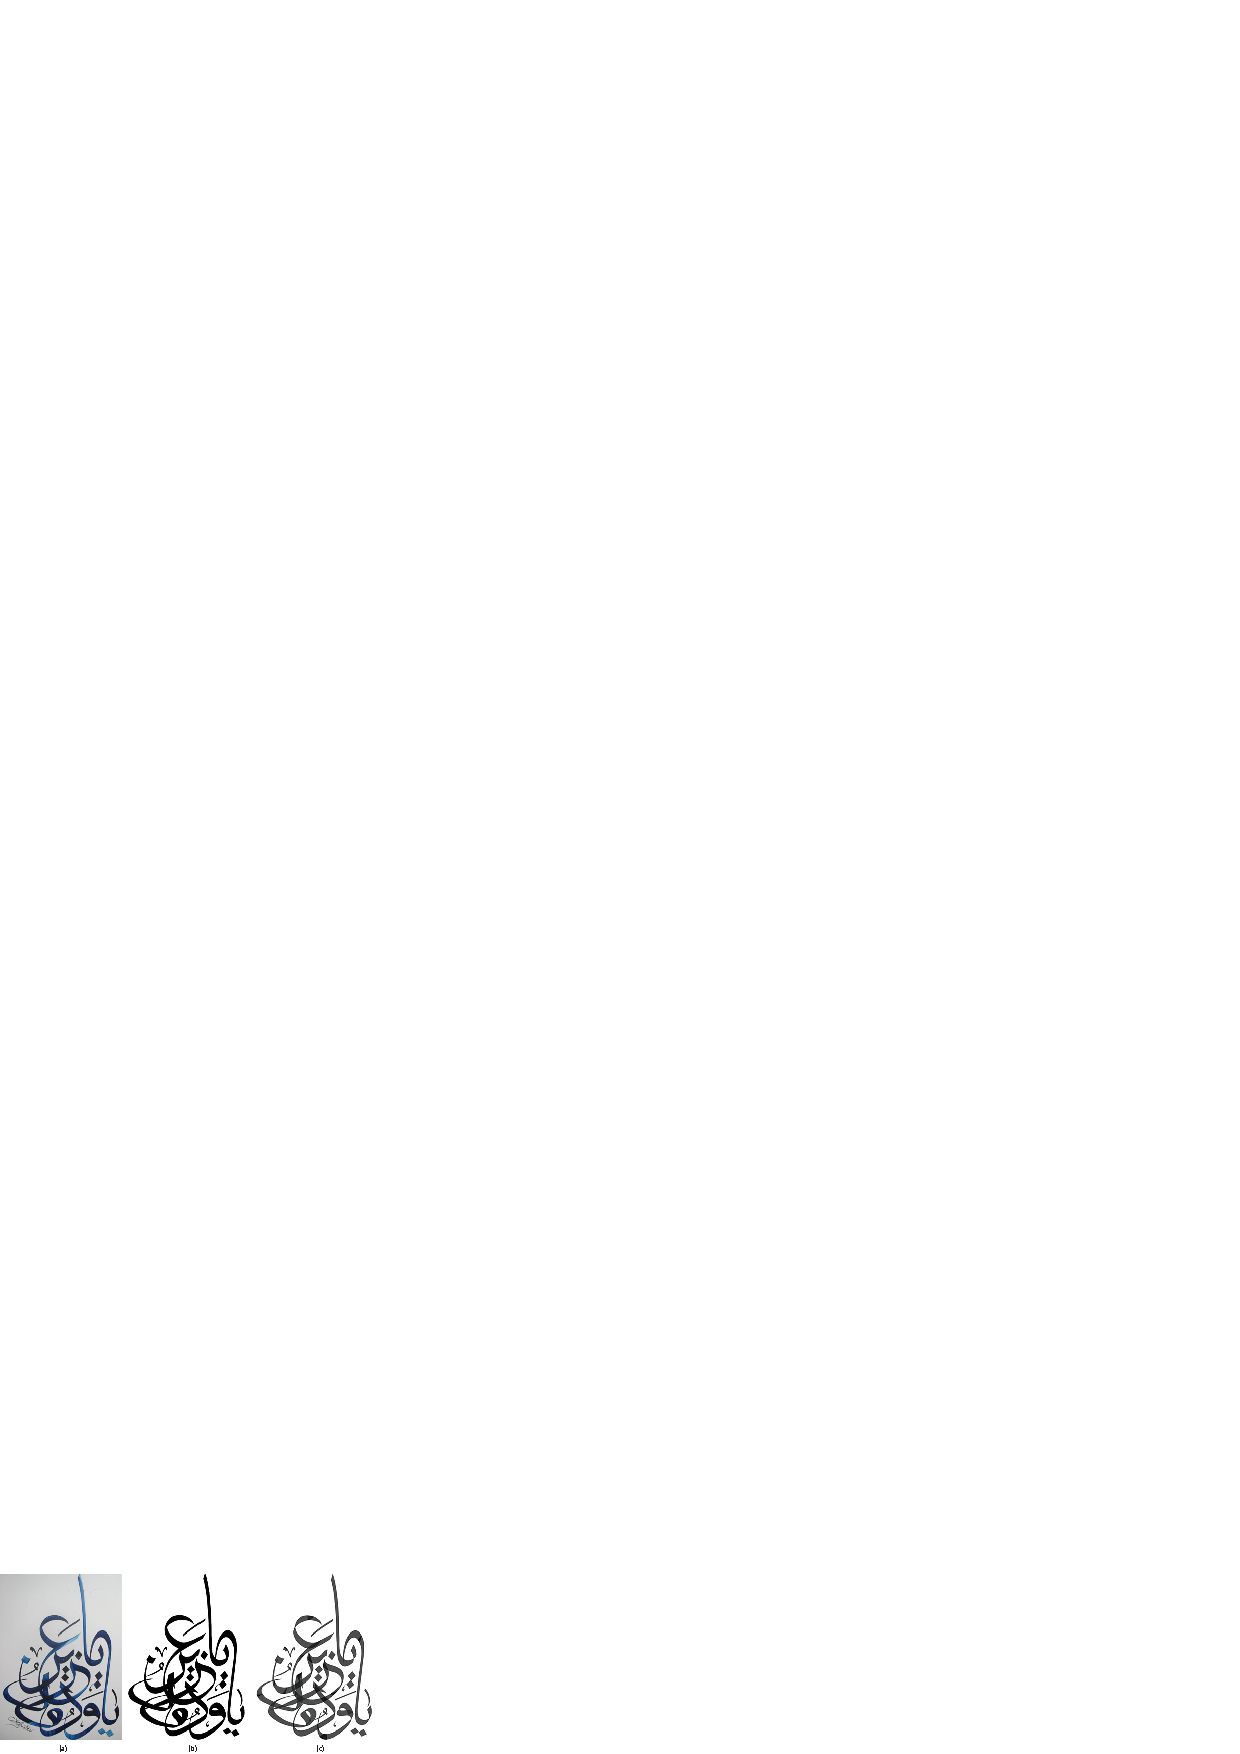
\includegraphics[width=2.5in]{../Images/ThuluthSample.pdf}
    \caption{
        A specimen produced in ``Thuluth'' script. (a) Original photograph of the specimen (b) Rasterized binary image of the twisting spline curves. (c) Rasteriezd shaded image of the twisting spline curves highlighting individual curve parts.
    }
  \label{Fig:Thuluth}
\end{figure}

\subsubsection{Machine Data Generation and Simulation}
    To check how accurately the data generated by these splines can be traced by an actual robotic manipulator, a computer simulation was used. We use an open-source simulator, developed  tailor made for the task. The simulator assumes an open loop [type] robot powered by stepper motors with controllable step size. To generate machine data, the simulator first rasterizes the whole spline with a variable resolution such that the distance between two adjacent points is always smaller than and required linear resolution. To fulfil this requirement for a point $N + 1$ on the discrete spline, the program iterates the fraction $f$ in the spline model [how do we refer to multiple equations?] to minimizes the error between the required resolution and the linear distance between $N$ and $N + 1$. For each computed $f$, the program then calculates the twist component. The set of these the two coordinates of each computed point and the twist component against $f$ defines the position and twist about the normal axis for the tool. The program then transforms this rasterized curve on to an emulated flat writing surface placed in a three dimensional space with some user-set position and orientation. To switch from one spline to the other, the program also adds some additional target points in the array of these points that will lift the tool normally upwards from the writing surface. Finally, the simulator tries to travel on this array of points at a constant speed.

    [Description 1]
    To emulate the writing pen, whenever the simulator detects that the distance of the tip of the tool lies within a configurable thin range, the program records the position and the twist component of the tool on every simulation step. The array of these points is connected using a $3$~D polygon that can be visualised on the screen. The $2$~D projection of this polygon on to the writing pad is extracted to be processed for the pixel-to-pixel comparison with the original script and the ideal rotating spline. The summary of these tests is shown in Table \ref{Table:MachineDataMetrices}.

    [Alternate shorter description]
    For the sake of analysis, in parallel, the end effector orientation is captured continuously to construct an ink mark with each sweep of the tool. The reproduced image is then used for analysis. The results of such a comparison can be seen in Table \ref{Table:MachineDataMetrices}.

    \begin{table}
    \begin{center}
    \caption{Benchmark of the mathematical accuracy of the twisting bezier spline curves with a simulated manipulator}
    \label{Table:MachineDataMetrices}
    \begin{tabular}{| c | c | c | c |}
    \hline
      & \textbf{Reference} & \textbf{Coverage} & \textbf{Extra} \\
      \hline
      \multicolumn{4}{|l|}{\textbf{Nastaleeq}}\\
      \hline
      Rotating Bazier Spline & Original Image & 95.8\% & 5.4\% \\
      \hline
      Machined Output & Original Image & 96.7\% & 7.0\% \\
      \hline
      Machined Output & Rasterized Image & 96.7\% & 4.3\% \\
      \hline
      \multicolumn{4}{|l|}{\textbf{Thuluth}}\\
      \hline
      Rotating Bazier Spline & Original Image & 93.4\% & 2.8\% \\
      \hline
      Machined Output & Original Image & 95.0\% & 3.4\% \\
      \hline
      Machined Output & Rasterized Image & 97.8\% & 4.4\% \\
    \hline
    \end{tabular}
    \end{center}
    \end{table} 